\DiaryEntry{Priority Queues}{2020-02-19}{Algorithms}

The heapsort algorithm can be extended to provide a priority queue: A priority queue maintains a set $\Sc$ of elements, each with an associated value called a key. A max-priority queue supports the following operations:

\begin{itemize}
\item Insert a new element with key $x$ into the queue.
\item Return the maximum value of the queue.
\item Remove and return the maximum value of the queue.
\item Increase the key of $x$'s key to value $k$.
\end{itemize}


\paragraph{Return Heap-maximum.} The heap-maxmum is simply the first element A[1].

\begin{verbatim}
heap-maximum(A)
    return A[1]
\end{verbatim}


\paragraph{Remove and Return Heap-Maximum.} We obtain the heap-maximum as above; however, in addition, we replace A[1] with A[heapsize] and heapify the heap.

\begin{verbatim}
heap-extract-max(A)
    max = A[1]
    A[1]=  A[heapsize]
    heapsize--
    max-heapify(A,1)
\end{verbatim}


\paragraph{Increase Key.} Here the key is updated and then the algorithm traverses a path from the corresponding element to the tree root. Along the way it exchanges the element with its parent, if the element is larger than the parent until is has found the correct place.

\begin{verbatim}
heap-increase-key(A,i,key)
    A[i] = key
    while(i>1) and A[Parent(i)] < A[i])
        exchange A[i] with A[Parent(i)]
        i = Parent(i)
\end{verbatim}

\paragraph{Insert a New Element.} We increase the heapsize and use the increase key algorithm to assign the ``right'' value to the newly inserted key.

\begin{verbatim}
insert(A,key)
    heapsize++
    A[heapsize] = -infinity
    heap-increase-key(A,heapsize,key)
\end{verbatim}


\subsection{Example}

We start with the queue shown in the following.

\begin{figure}[H]
\centering
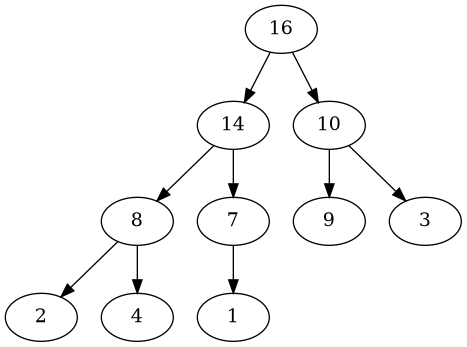
\includegraphics[scale=0.5]{images/heap_queue_01.png}
\end{figure}

Removing and returning the heap-maximum yields the following tree. Compare to before, node $14$ has now node $10$ as child. This causes the reorganization of the left subtree (e.g. node $1$ moved to the left).

\begin{figure}[H]
\centering
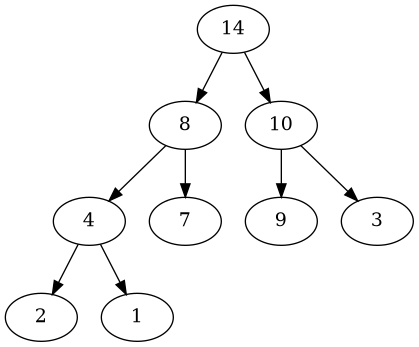
\includegraphics[scale=0.5]{images/heap_queue_02.png}
\end{figure}

Now let's increase node id $9$ (having value $1$) to value $12$. This yields the following tree.


\begin{figure}[H]
\centering
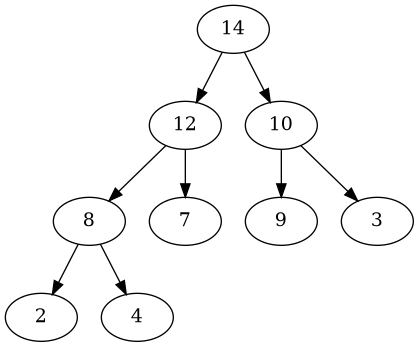
\includegraphics[scale=0.5]{images/heap_queue_03.png}
\end{figure}

And finally, let's insert the value $100$ into the queue. We obtain the following tree.

\begin{figure}[H]
\centering
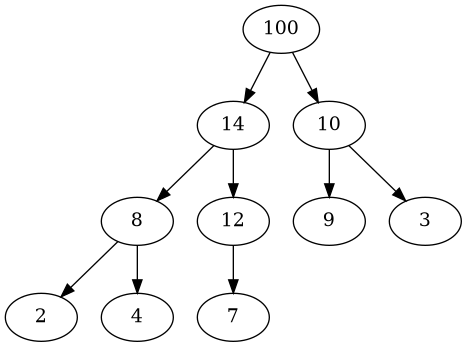
\includegraphics[scale=0.5]{images/heap_queue_04.png}
\end{figure}

Note: Not $100\%$ sure here, but I think the tree fulfills the max-heap property. Every parent is larger than its children; that node $12$ is ``below'' node $10$ is ok, as node $12$ parent (node $14$) is larger then $12$.

%%% Local Variables:
%%% mode: latex
%%% TeX-master: "journal"
%%% End:
